\subsection{Creating a project}
\begin{itemize}
	\item{Navigate to projects list page}
	\newline
	After you have signed in you will be navigated to the projects list page, if you wish to navigating there from another page, you can simply click on the projects tab on the left side navigation bar.
	\begin{figure}[H]
	    	\centering
	    	\fbox{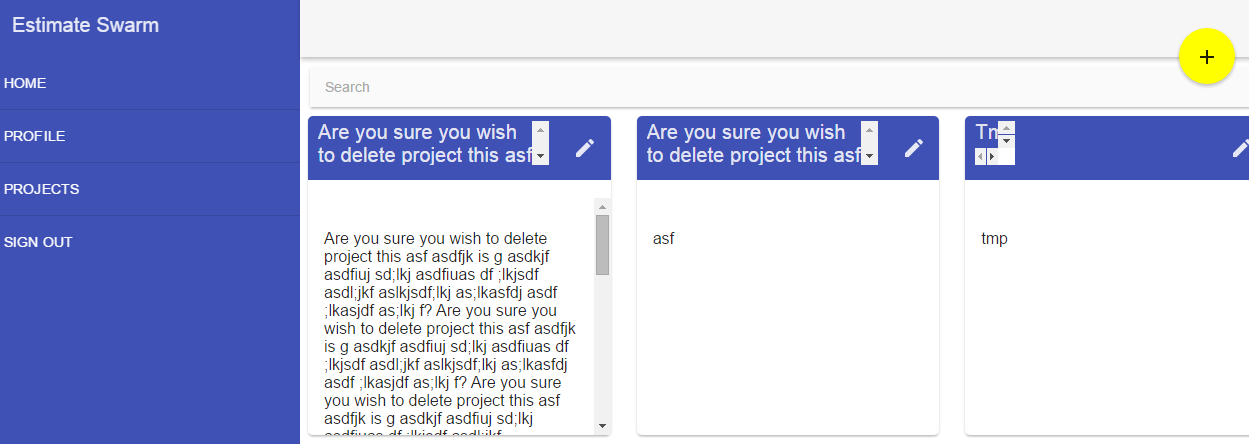
\includegraphics[width=0.5\textwidth]{projectsList}}
	    	\caption{Projects List Page}
	    	\label{fig:Learning rate 0.1}
   	\end{figure}
	\item{Add a new project}
	\newline
	On the projects list page, you can simply click on the "add project" button that is in the top right hand corner of the screen.
	\begin{figure}[H]
	    	\centering
	    	\fbox{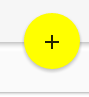
\includegraphics[width=0.5\textwidth]{addButton}}
	    	\caption{Add Project Button}
	    	\label{fig:Learning rate 0.1}
   	\end{figure}
	\item{Complete details of the project}
	\newline
	On the "Create Project" page you will have to fill in the details of the project in order to complete the creation of the project. You will have to give the project a name and a description. You will also have to indicate who will be allowed to estimate on the project as shown in the figure below.
	\begin{figure}[H]
	    	\centering
	    	\fbox{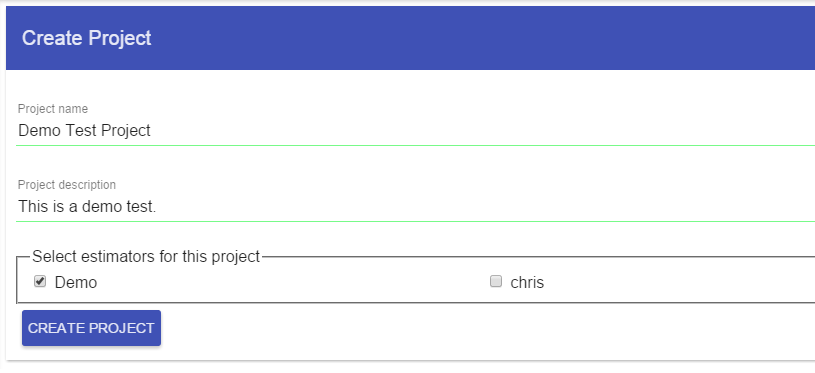
\includegraphics[width=0.5\textwidth]{createProj}}
	    	\caption{Create Project Page}
	    	\label{fig:Learning rate 0.1}
   	\end{figure}
\end{itemize}
\subsection{Estimation Process}
\begin{itemize}
	\item{Create Project Tree}
	\newline
	From here you will have to create a project tree that represents the project that you need an estimation on. You can do this by adding features, this is done by clicking the "Add feature" button, once this is done each feature can be expanded further by clicking on the "+" button on the individual nodes. Features can then be given a name, represented by the title field and a description. You can save the tree by clicking on the "Save Project" button to continue editing the tree at a later point. When you are satisfied with the tree, you can open it for estimation, by clicking on the "Open For Estimation" button. After the project has been opened for estimation, it can not be edited again. Emails will be sent out the users that were chosen to estimate on the project to inform them that the project is now available for estimation.
	\begin{figure}[H]
	    	\centering
	    	\fbox{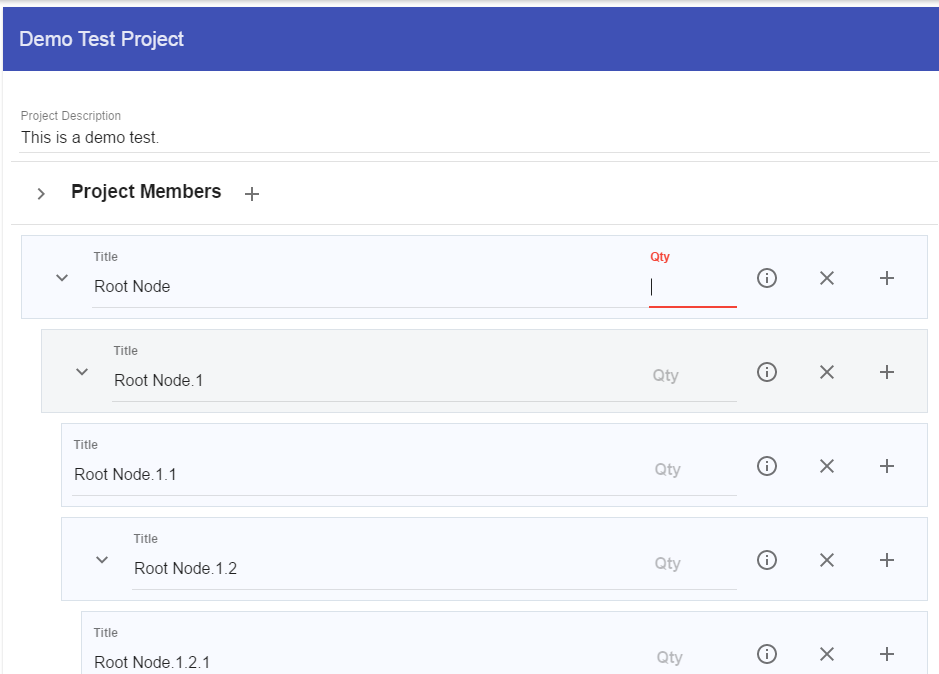
\includegraphics[width=0.5\textwidth]{createTree}}
	    	\caption{Create Tree Page}
	    	\label{fig:Learning rate 0.1}
   	\end{figure}
	\item{Estimating}
	\newline
	The estimators can now estimate on each of the leaf nodes of the project. The values on the leaf nodes then bubble up to their respective parent nodes. The values in the "Project Estimation Total" list reflect the total estimations for the entire project for the current estimator. When the estimator is done, he/she can click on the "Submit Estimation" button to submit his/her estimation to the project owner.
	\begin{figure}[H]
	    	\centering
	    	\fbox{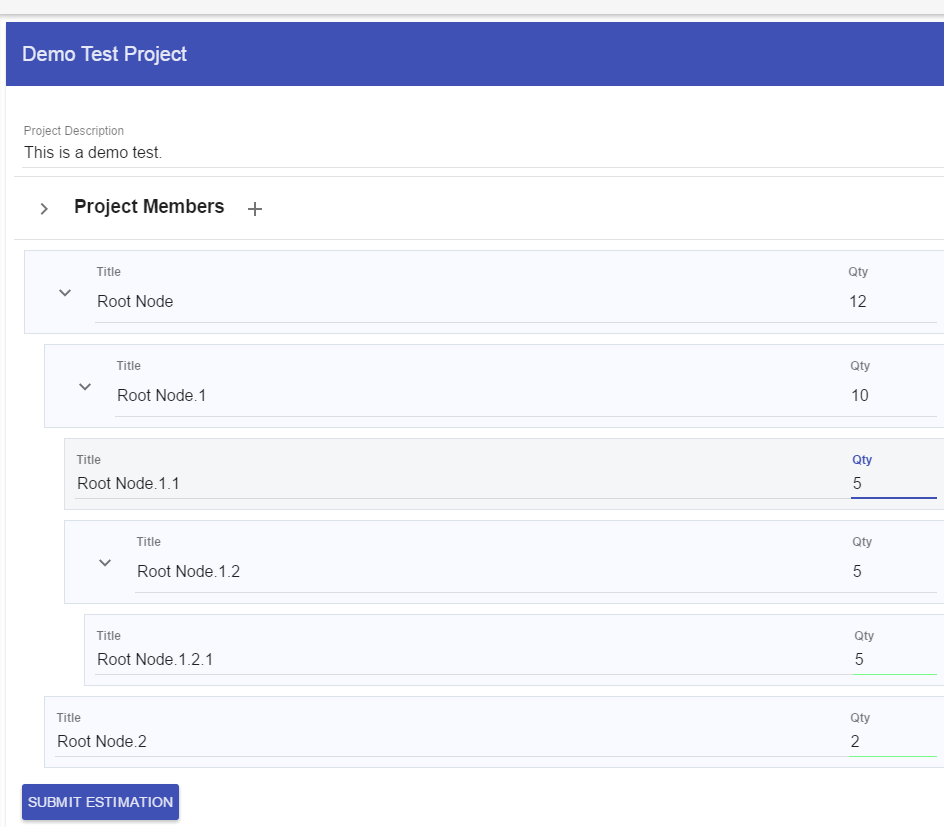
\includegraphics[width=0.5\textwidth]{estimate}}
	    	\caption{Estimation Page}
	    	\label{fig:Learning rate 0.1}
   	\end{figure}
\end{itemize}
\subsection{Reports}
After the estimation has been completed a report will be generated based on the current structure of the project. This report will automatically provide you with four graphs. each graph deals with a different aspect of the Delphi Wide Band method. 
\begin{itemize}
	\item{Bar Graph}
		\begin{figure}[H]
	    	\centering
	    	\fbox{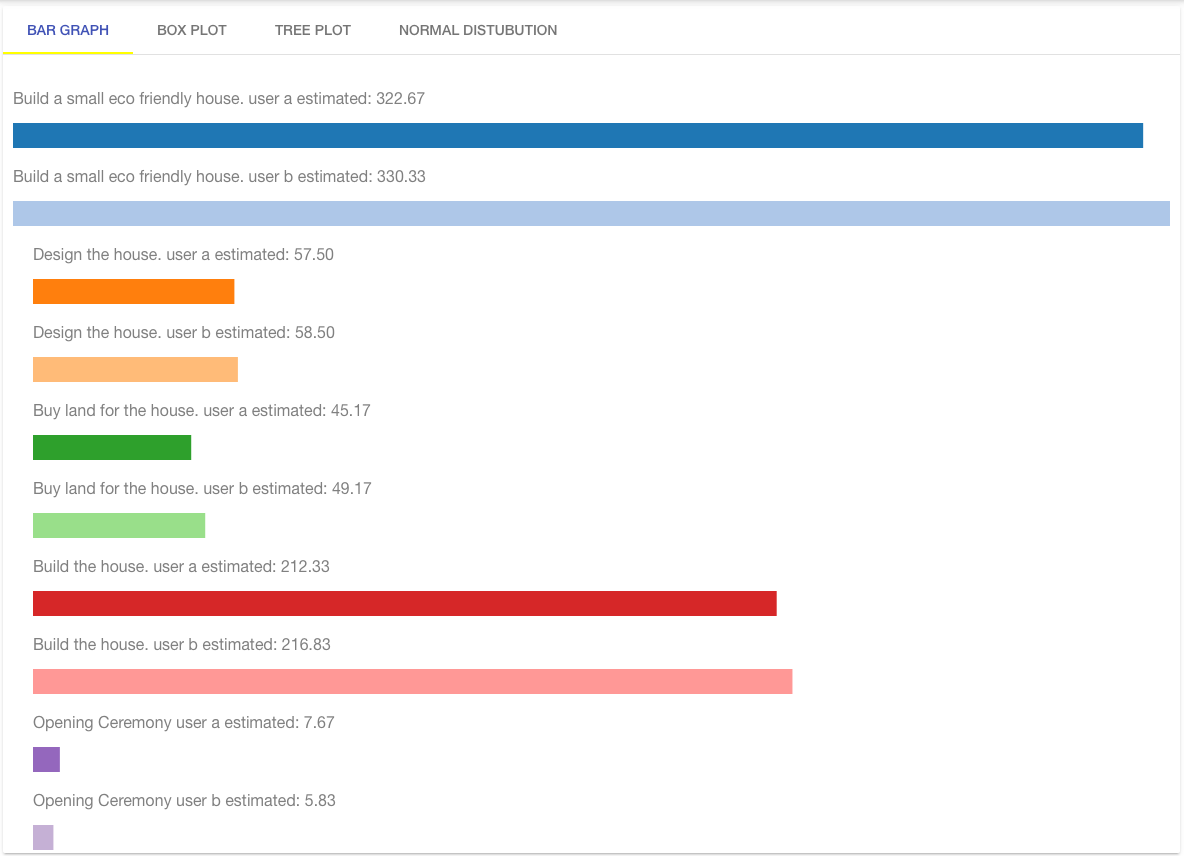
\includegraphics[width=0.5\textwidth]{bargraph}}
	    	\caption{Bar Graph}
	    	\label{fig:Bar Graph}
   	\end{figure}
	The purpose of the bar graph is to give a user the indication of who has estimated what value. Each estimator's estimation will be indicated as a bar. The bar graph also indicated the structure of the project. 
	\item{Box Plot}
	\begin{figure}[H]
	    	\centering
	    	\fbox{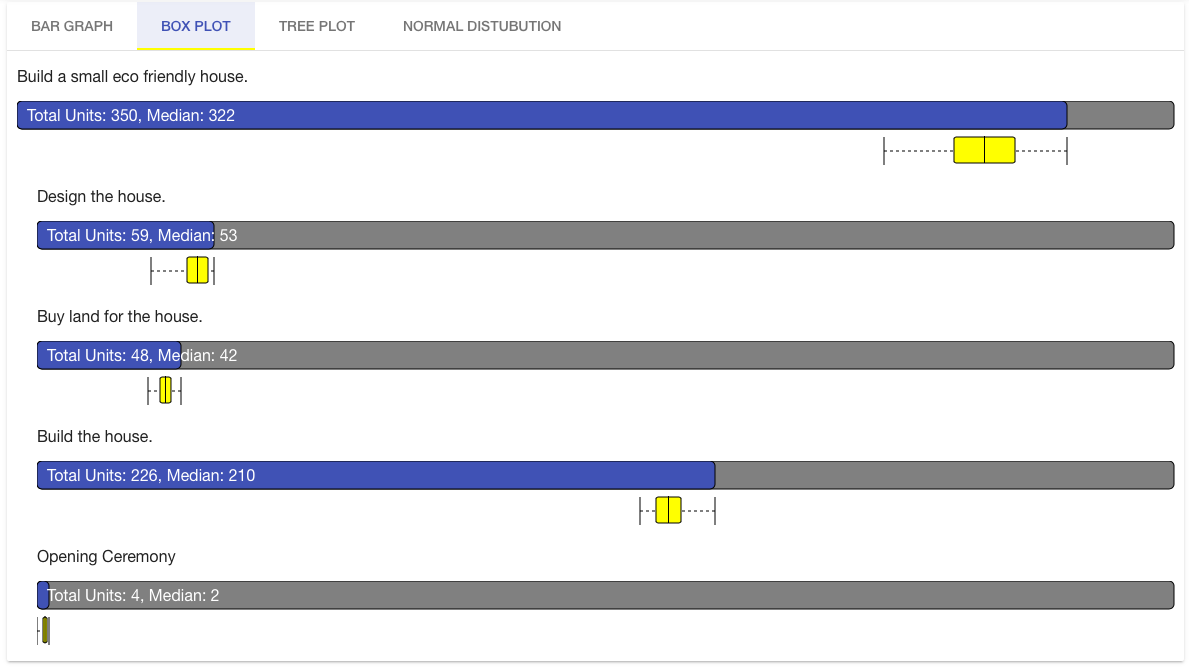
\includegraphics[width=0.5\textwidth]{boxplot}}
	    	\caption{Box Plot}
	    	\label{fig:Box Plot}
   	\end{figure}
	The purpose of the box plot is to show each item in the project tree and indicate if users are estimating the same amount or not. The box plot that have small whiskers indicate that the users generally agree on a item. If a whisker does not fall outside the box plot it indicates that all estimations are within one standard deviation of the mean(Average). The box plot also makes use of a bar graph to indicate what the mean is and how much a particular item is contributing to the main goal of the project.
	\item{Tree Plot}
	\begin{figure}[H]
	    	\centering
	    	\fbox{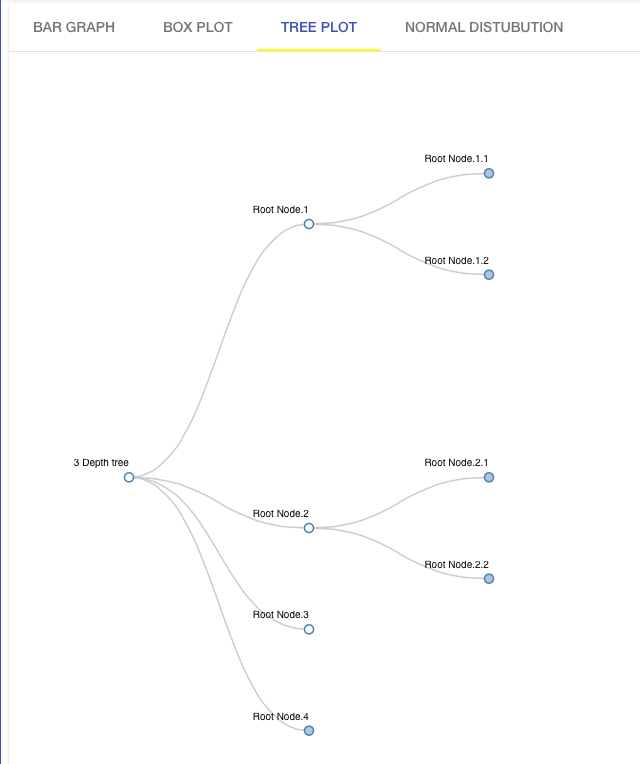
\includegraphics[width=0.5\textwidth]{treeplot}}
	    	\caption{Tree Plot}
	    	\label{fig:Tree Plot}
   	\end{figure}
	The Tree Plot is a collapsable and expandable graph of the tree's structure. it purpose is to allow a user to interrogate a specific aspect of the project. These interrogations will generally lead to a indication of where problems lies in a project. Nodes can be collapsed and expanded as the user requires it. 
	\item{Delphi Wide Band Normal Distribution}
	\begin{figure}[H]
	    	\centering
	    	\fbox{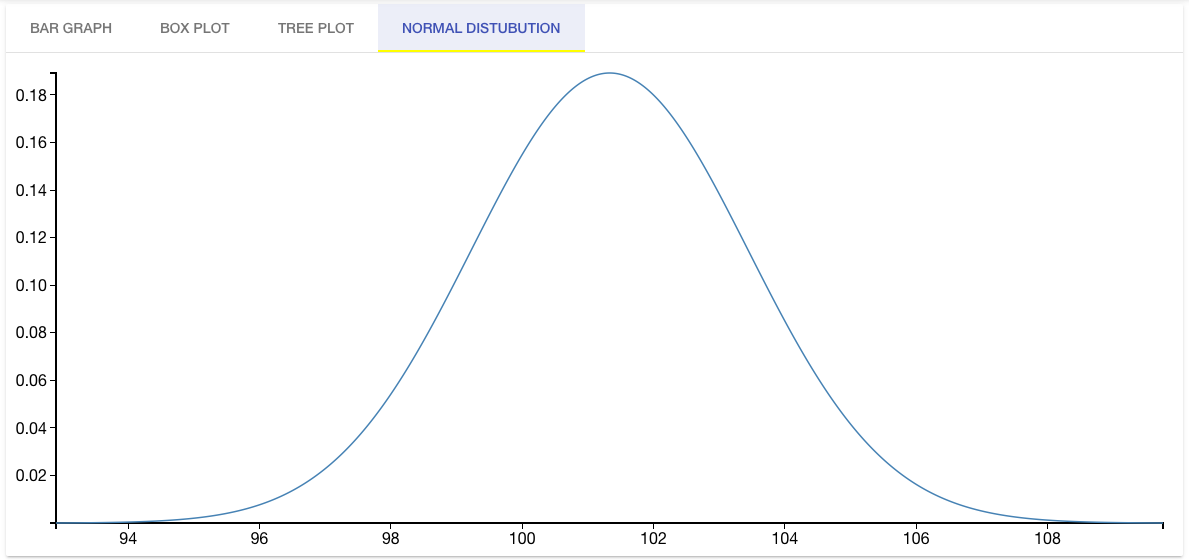
\includegraphics[width=0.5\textwidth]{normaldist}}
	    	\caption{Delphi Wide Band Normal Distribution}
	    	\label{fig:Delphi Wide Band Normal Distribution}
   	\end{figure}
	The normal distribution is a important part of the delphi wide band method. It indicates to the user if there is consensus regarding project as a whole. Typically a value between 10 percent to 20 percent indicate that the users have consensus. Anything lower than 10 percent indicate that there is still room for improvement. The higher the value of the y axis is the closer estimations are grouped together. The lower y axis value is the estimations is spread out and generally users do not agree on particular project.
\end{itemize}
\subsection{Organisations}
Organisations can be used to group related projects or divisions of a company. This helps the user to not  be overwhelmed by the sheer number of estimators/projects. Only relevant information for a user is displayed. This increases the usability of the system dramatically. Users can be part of multiple organisations or they can belong to no organisation at all. This allows the estimation system to scale from big to small companies as required. We can create organisations under the organisation tab and selecting the add organisations FAB button.
	\begin{figure}[H]
	    	\centering
	    	\fbox{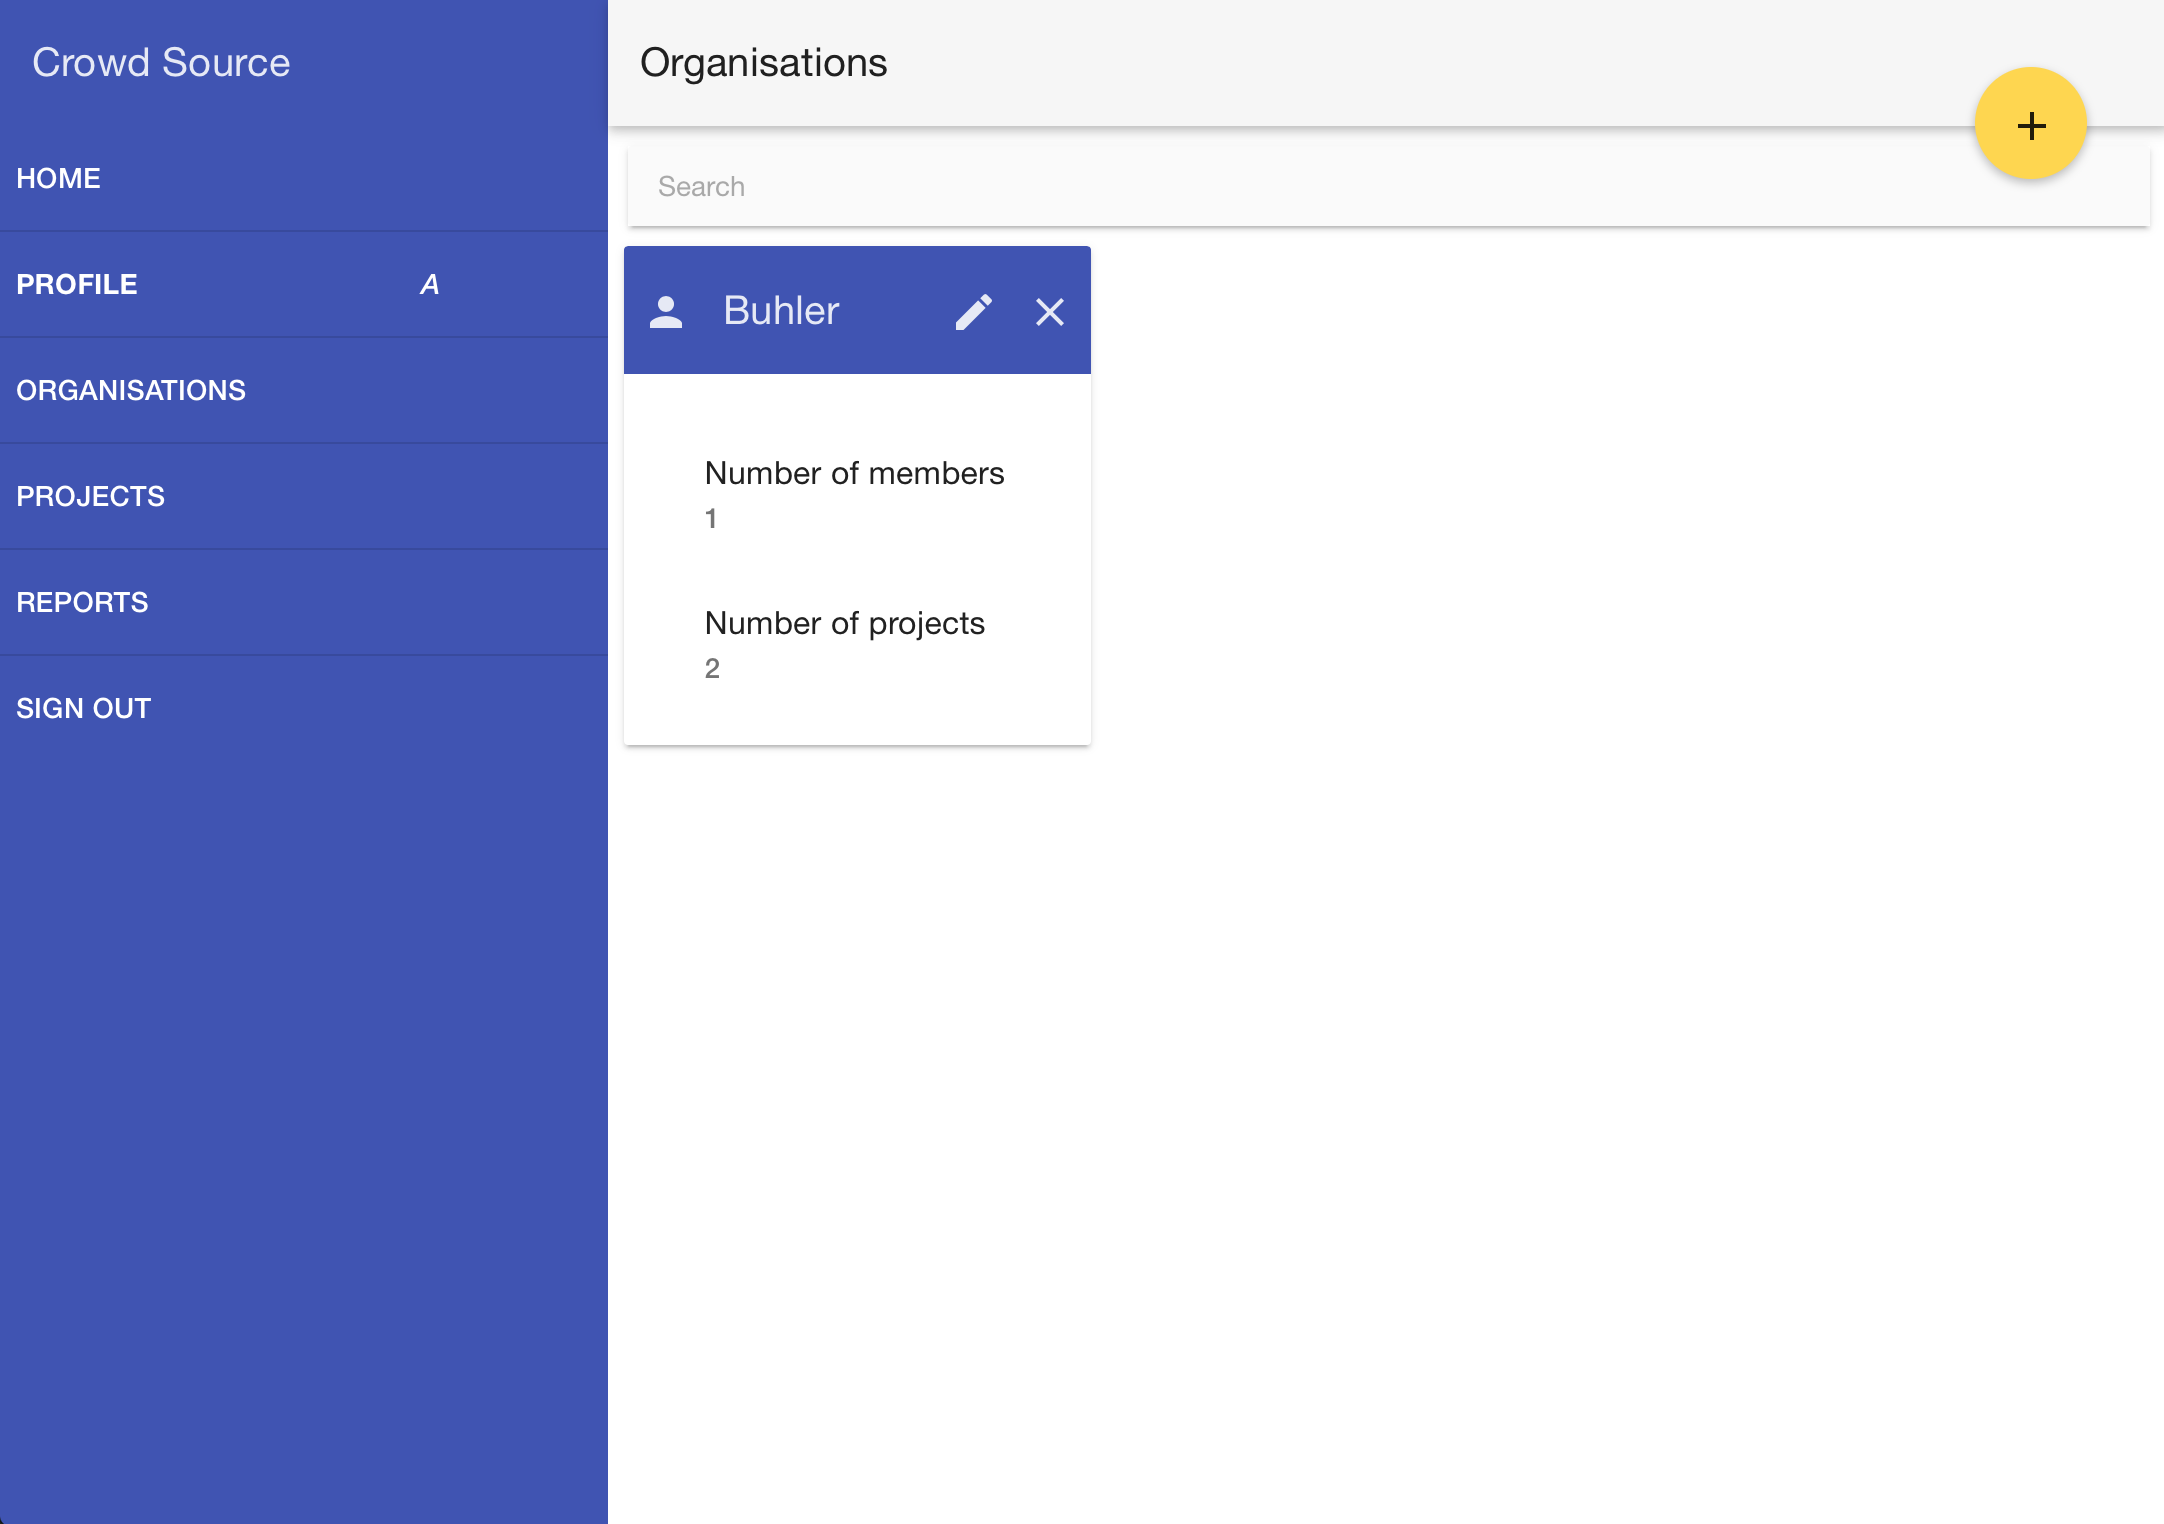
\includegraphics[width=0.5\textwidth]{AddOrg}}
	    	\caption{Add Organisation}
	    	\label{fig:Add Organisation}
   	\end{figure}
After creating a organisation you will be promoted to choose a name for the organisations and which members belong to this organisation.
	\begin{figure}[H]
	    	\centering
	    	\fbox{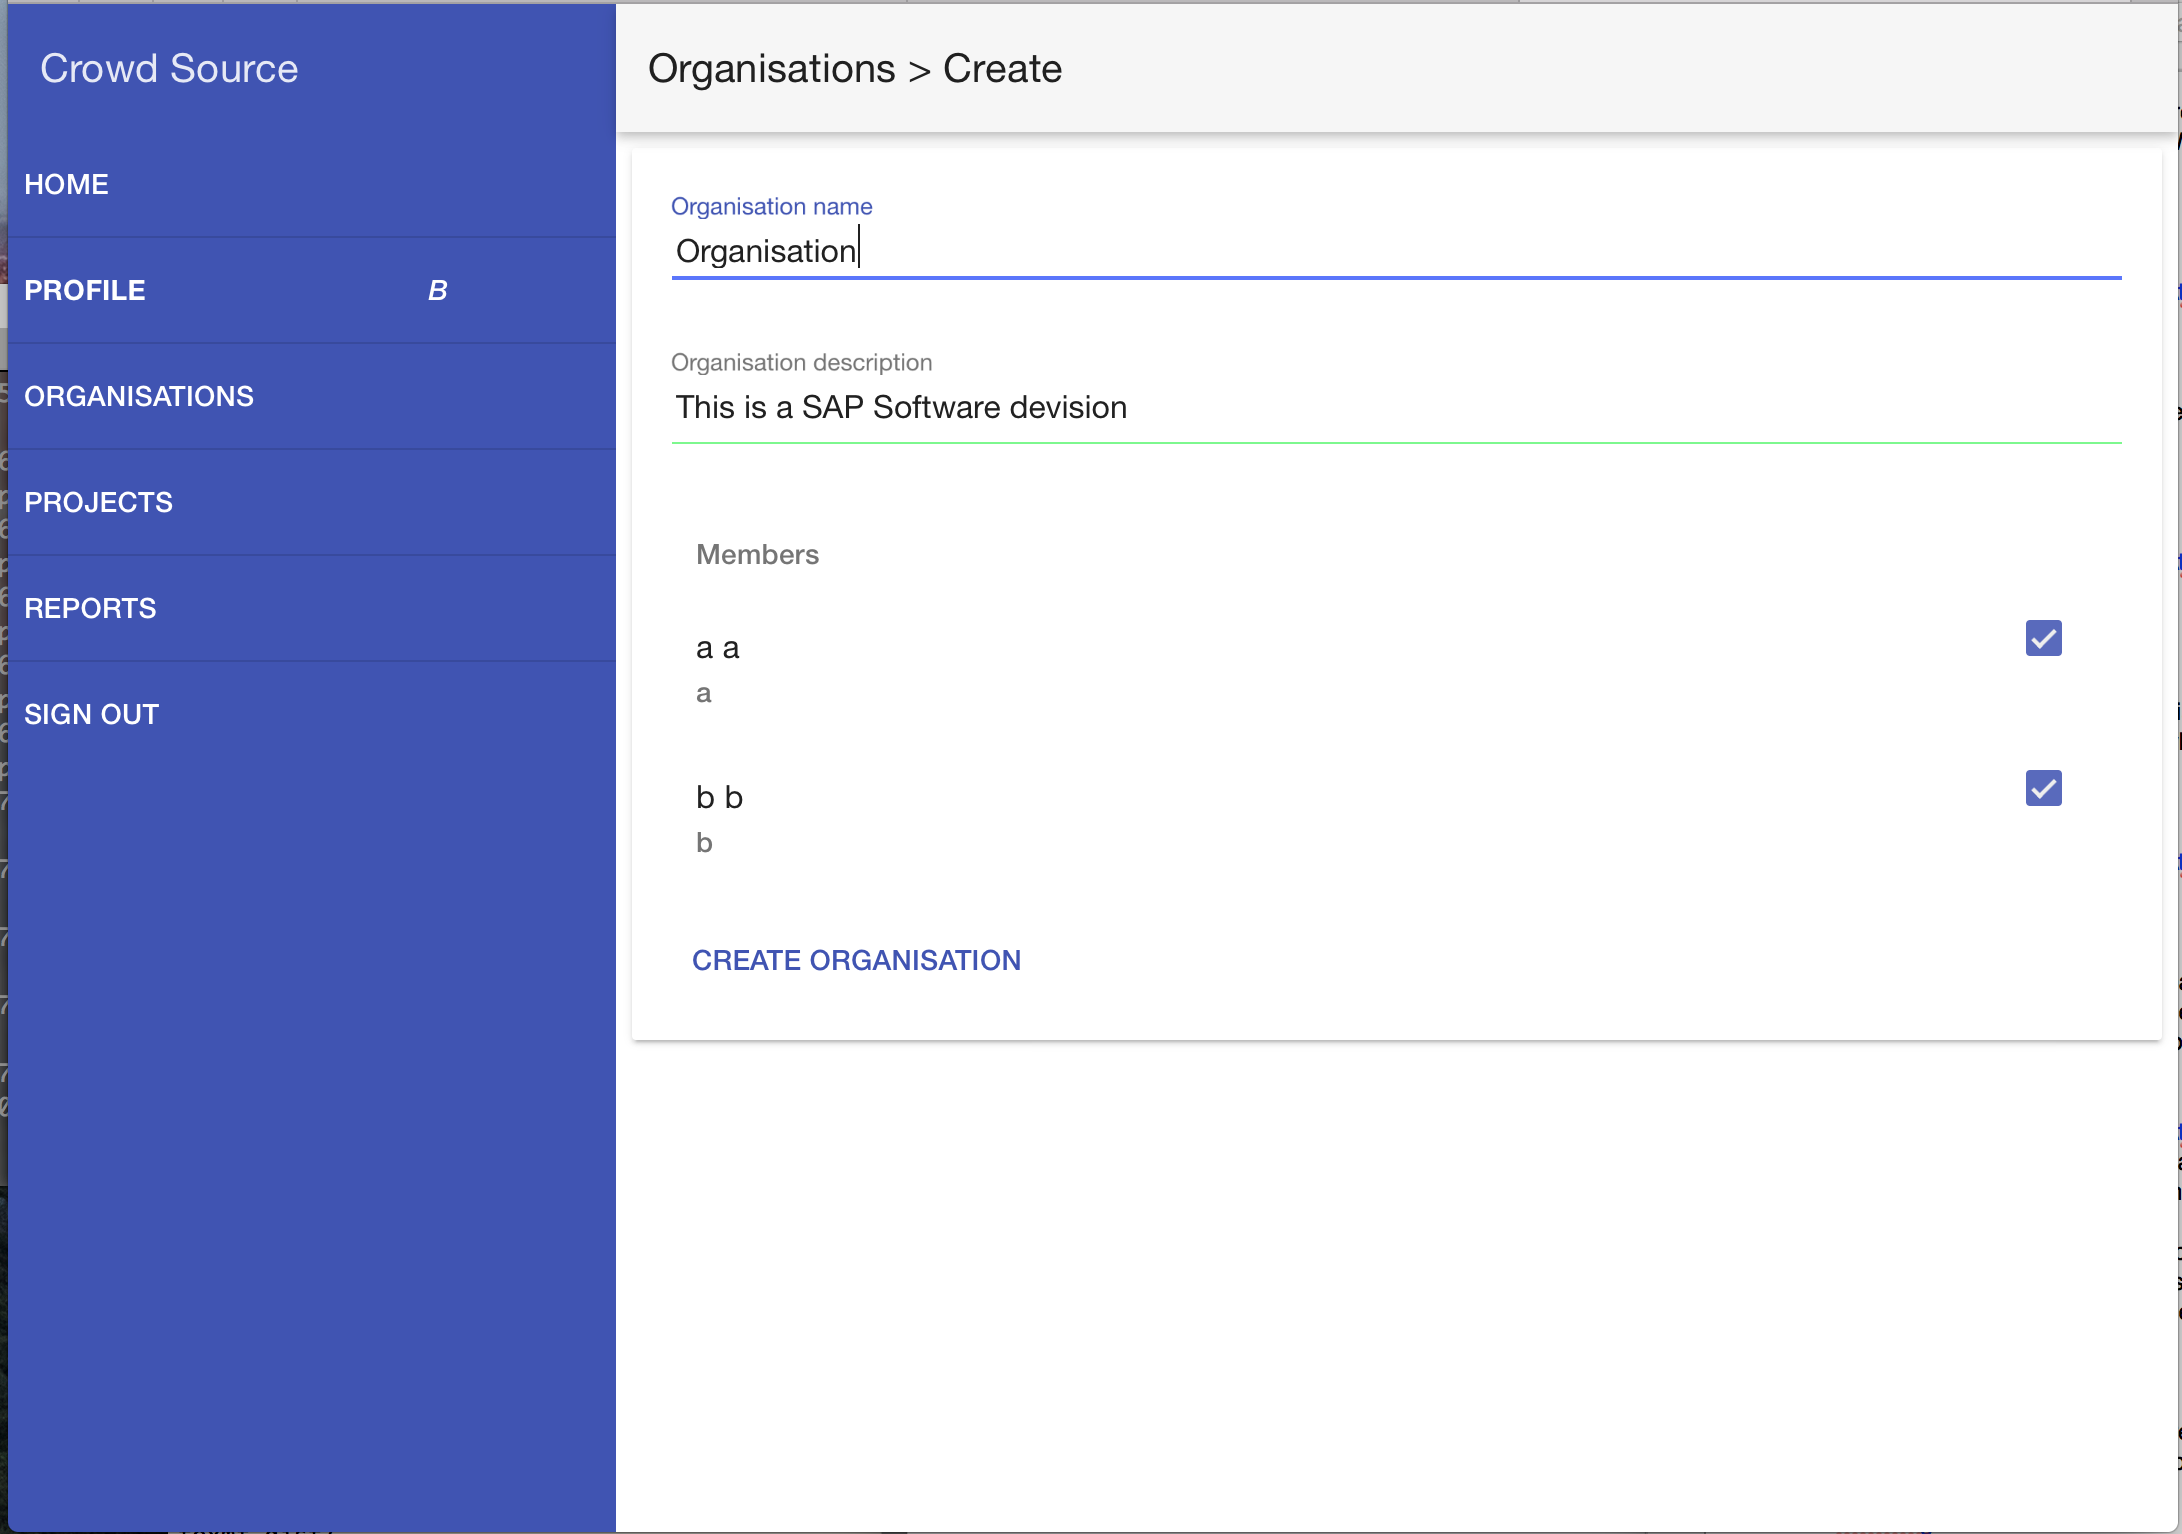
\includegraphics[width=0.5\textwidth]{SetupOrg}}
	    	\caption{Add Details to Organisation}
	    	\label{fig:Add Details to Organisation}
   	\end{figure}
After the project has been created a project can easily be assigned to the organisation. This is done in the project creation process as described in this manual.  Viewing a organisation will show which members are assigned to a particular organisation and they can be added or removed. 
	\begin{figure}[H]
	    	\centering
	    	\fbox{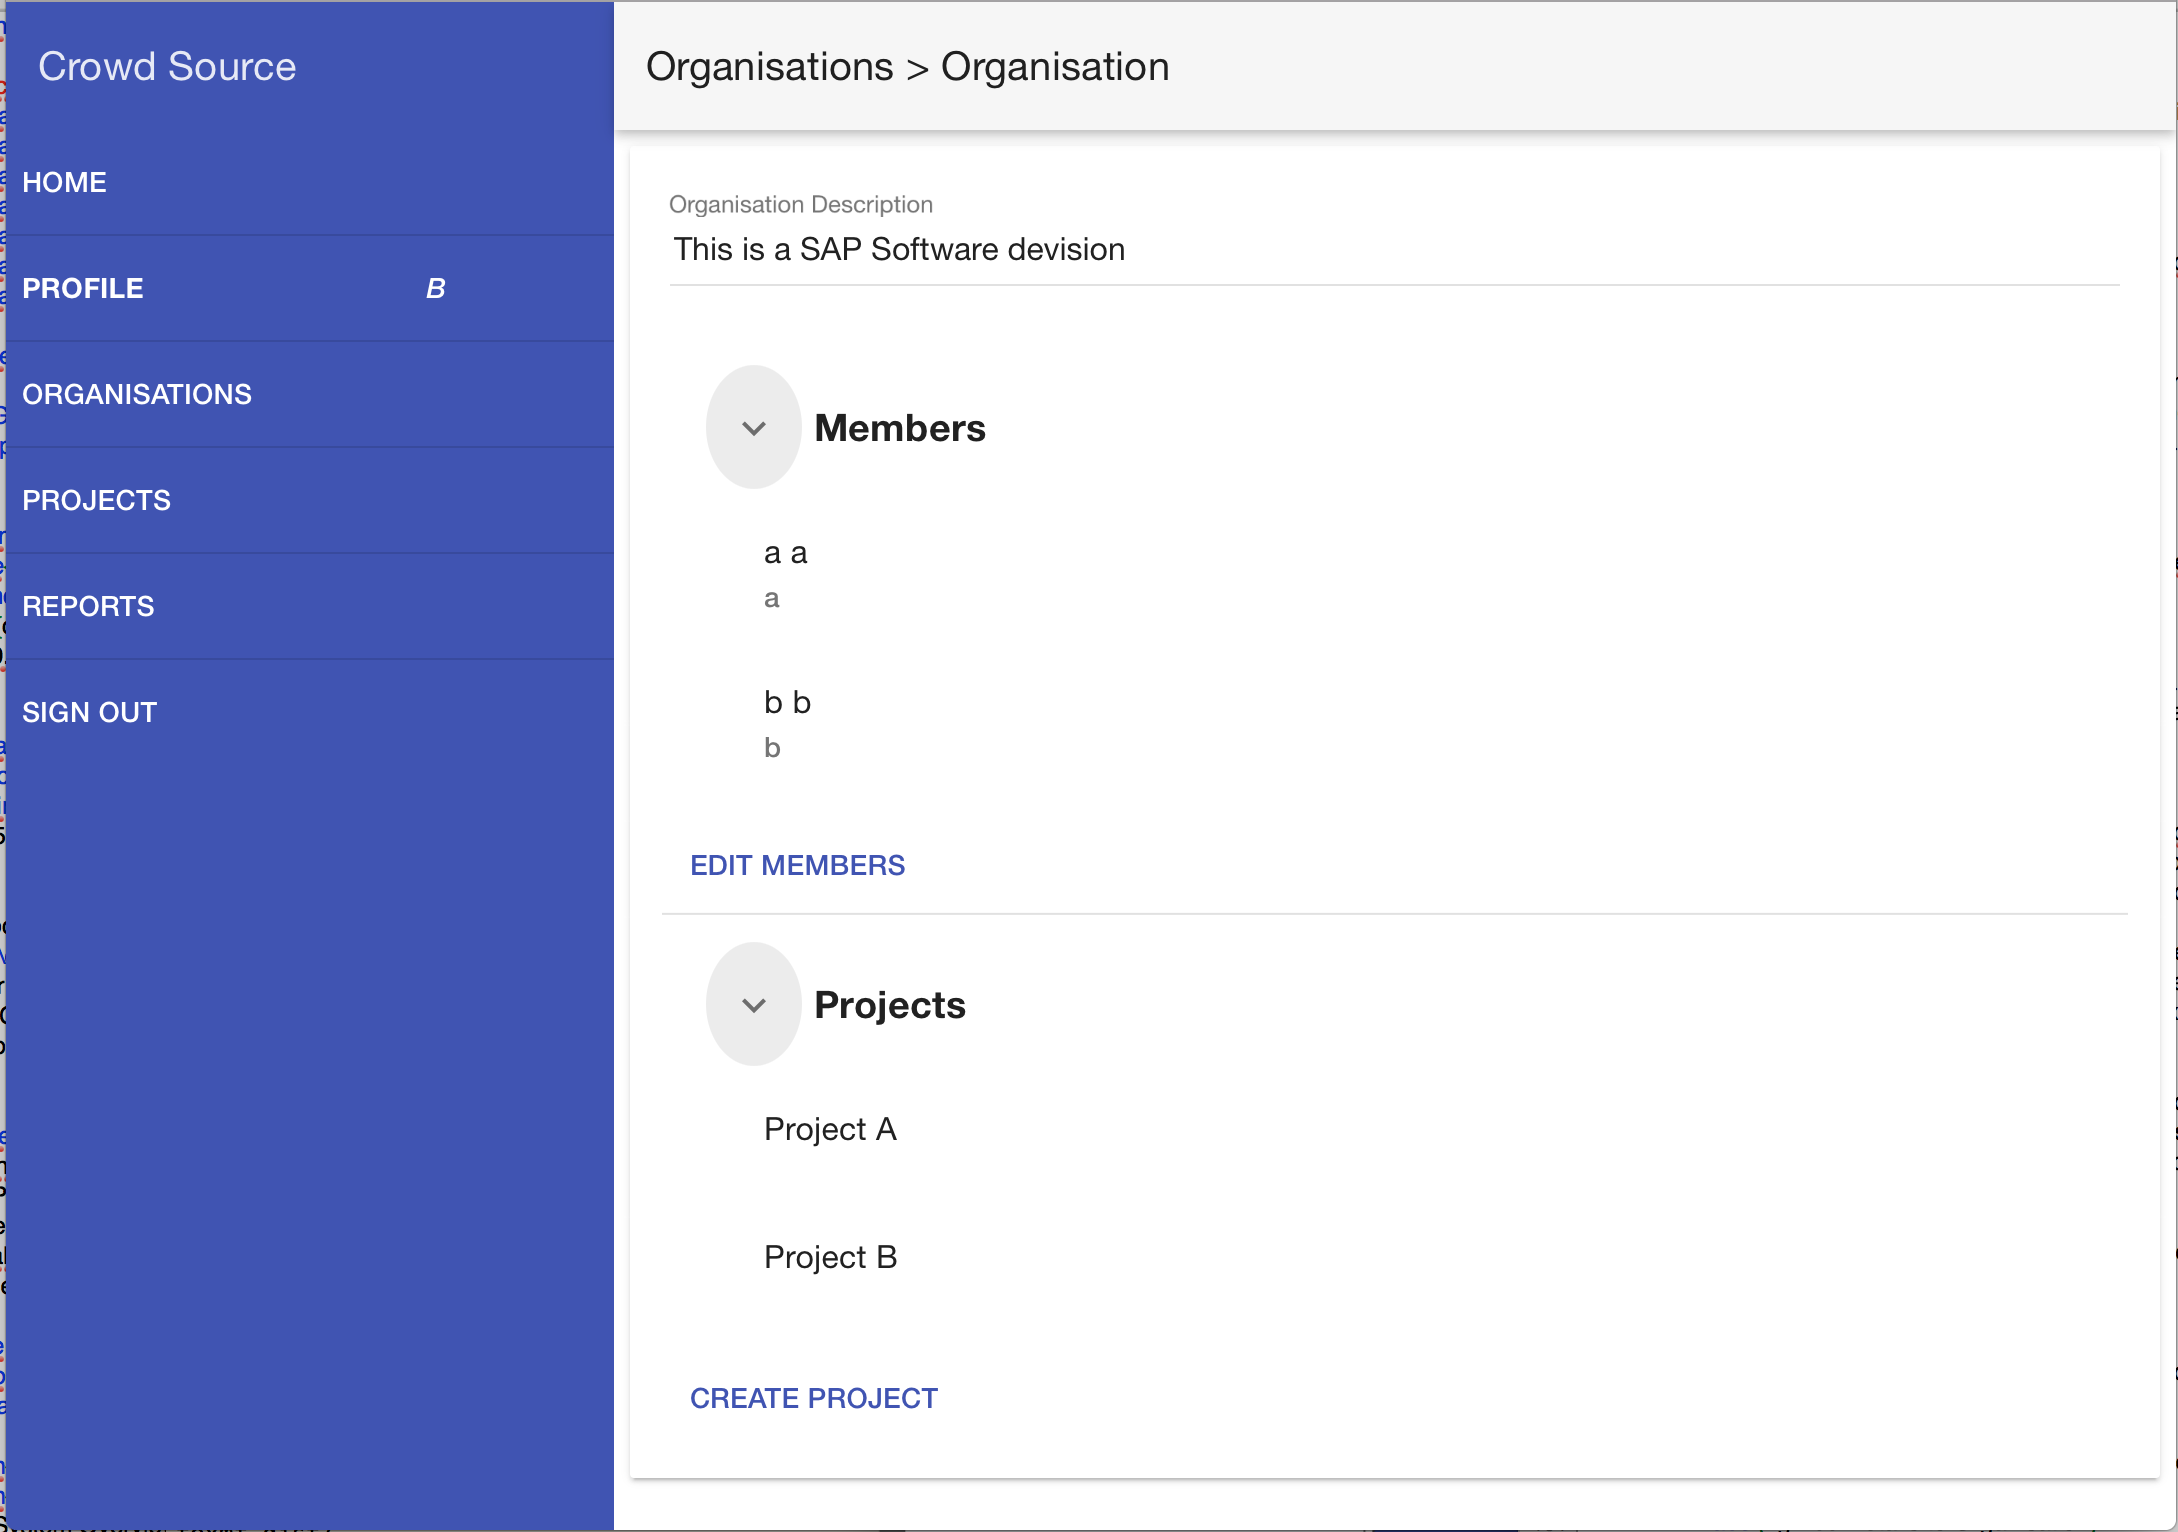
\includegraphics[width=0.5\textwidth]{DetailOrg}}
	    	\caption{Details of Organisation}
	    	\label{fig:Details of Organisation}
   	\end{figure}
	
	
	
	
	
	
	
	
	
	
	
	
	
	
	
	
	
	
	
	
	